% Please use the skeleton file you have received in the
% invitation-to-submit email, where your data are already
% filled in. Otherwise please make sure you insert your
% data according to the instructions in PoSauthmanual.pdf
\documentclass{PoS}
\usepackage{subfig}
\everymath{\displaystyle}

\title{Gamma-ray Pulsars with DAMPE}

\ShortTitle{Gamma-ray Pulsars with DAMPE}

\author{\speaker{Maria Munoz}\\
        University of Geneva, Geneva, Switzerland\\
        E-mail: \email{maria.munoz@unige.ch}}

\author{Xin Wu\\
        University of Geneva, Geneva, Switzerland}
\author{Fabio Gargano\\
        INFN, Bari, Italy}
\author{Kai-Kai Duan\\
        Purple Mountain Observatory, Nanjing, China}
\author{Zhao-Qiang Shen\\
        Purple Mountain Observatory, Nanjing, China}
\author{on behalf of the DAMPE collaboration}

%\author{Another Author\\
%        Affiliation\\
%        E-mail: \email{...}}

\abstract{The DArk Matter Particle Explorer (DAMPE) is a satellite-borne experiment successfully launched in December 2015.  DAMPE has been taking data for over 3.5 years during which it has been observing the full gamma-ray sky above 1 GeV. The data used for this contribution considers the first 2 years of data and within an energy range from 2 GeV to 100 GeV.   Among all the pulsars observed by DAMPE we will present the measurement results for the 10 brightest gamma-ray pulsars which include Vela, Geminga and Crab. The light curves and energy spectra, including the phase averaged energy spectra will be presented for these 10 pulsars. From these results we will derive the timing precision of DAMPE, which is of importance for its other scientific goals, as well as the potential for future gamma-ray studies with DAMPE.}

\FullConference{36th International Cosmic Ray Conference -ICRC2019-\\
		July 24th - August 1st, 2019\\
		Madison, WI, U.S.A.}


\begin{document}

%\section{Introduction}

%Pulsars importance introduction

\section{Introduction}


The DArk Matter Particle Explorer (DAMPE) is China's first astronomical satellite launched the 17th of December 2015. DAMPE has been successfully taking data for over 3.5 years.
The satellite has a sun-synchronous orbit at an altitude of  500 km and  has a period of 95 minutes i.e. 15 orbits per day.
The instrument consists of four sub-detectors, from top to bottom: A Plastic Scintillator Detector (PSD) used as an anti-coincidence shield for photon identification and for charge measurement of heavy ions.
A Silicon TracKer(STK) composed by six double layers of silicon: the first three layers are inter-layered  by a tungsten layer to promote pair conversion of gamma-rays.  A BGO Calorimeter for energy measurements and separation of electromagnetic/hadronic showers with a depth of $\sim 32$ radiations lengths. Finally a NeUtron Detector (NUD) for  hadronic identification \cite{dampe-mision}.

One of the main scientific objectives of DAMPE is the detection and study of  high energy gamma-rays (above 1 GeV). One of the first detailed gamma-ray study using the DAMPE data focuses on pulsars. Pulsars are highly magnetized rotating neutron stars of great interest because of their characteristics. The time  properties of pulsars makes them very reliable sources for timing calibration. The observation of Pulsars by DAMPE contributes to two key calibration points of the instrument, the confirmation of gamma-ray detection and the  evaluation of the time  performance in DAMPE.
Previous searches of pulsars  in  $\gamma$-rays  with space-based experiments have been made for example  with   EGRET,AGILE and  FERMI\cite{2catalogfermi}, the latter still contributing to the discovery of $\gamma$-ray pulsars.


\section{Data Selection}

In a previous paper  a method for resolving gamma-ray events detected by DAMPE has been presented \cite{zunlei}, nevertheless for this work a different selection has been used. The reason for using a different selection is to increase our signal statistics at low energies to improve the detection of pulsars. As explained before, pulsars have a a very characteristics light curve and emission occurs at a defined known periodicity different  for each pulsar, therefore if the events detected are mistagged as photons they will over-all not contribute to the pulsar light curve measurements. Instead these events will smear-out into the background. Therefore for pulsar analysis a photon selection with a relatively higher electron contamination is permissible.
The steps for the gamma-ray identification are similar to those presented in \cite{zunlei},
\begin{enumerate}
	\item electron/proton separation: Using the BGO to search for characteristics signatures of electronic and hadronic shower, the objective is to reject hadrons. Knowing that $\sim 98\%$ of primary cosmic rays are hadrons it is important to reject them as first step.
	\item Use of the PSD as anti-coincidence shield, gamma-rays leave no signal in the PSD. This is essential for electron rejection.
	\item Search for tracks in the STK that interact after the first tungsten layer. To eliminate electrons and because of this cut we select only photons that convert within the STK.
	\item Alongside the previous cuts, we also apply geometrical cuts to reject events that arrive from the sides or bottom of the detector. Searching for a well contained shower in the BGO for reliable energy measurement and photon directionality.

\end{enumerate}

On top of the steps for photon identification, quality cuts are applied. First, events that cross the South Atlantic Anomaly are rejected. Lastly, the DAMPE instrument has a complex trigger system and an interacting particle can trigger one or more triggers, differentiation of this triggers is also taken into consideration. For this work we will focus on the Low Energy Trigger (LET) and the High Energy Trigger (HET). The HET has no pre-scale and as its name suggest is more efficient at higher energies. The LET is pre-scaled, meaning only a fraction of the events are stored,  and it varies depending on the position of the DAMPE with respect to Earth. The Low Energy Trigger has a lenient logic than the High Energy Trigger and therefore it has a pre-scaling dependent on the latitude, where for the low latitudes from -20 to 20 the pre-scale is set to 8 and for the other latitudes the pre-scale corresponds to 64.


%using the properties of the PSD as  an anti-coincidence  shield and further looking in the calorimeter for the signature  hadronic and electromagnetic showers to reject charge  firstly heavy ions.  Further for electron separation we search for  events that leave no track in the  STK before  the first tungsten layers therefore looking only for converted  photons.
The  result of this  selection can be observed in Figure \ref{eff_area}, where results are shown for the two different triggers. The dependency on energy and the incoming angle  of the photon in detector coordinates on the effective area are indicated.

The overall data set studied corresponds  $\sim 39$ months of observations. For  this period of time a total of  354,985 events have been detected. In Figure \ref{map} the gamma=ray sky as observed by DAMPE with the current selection for $\sim 39$ months is presented with an energy range from 1 GeV to 100 GeV


% The electron acceptance for this selection is shown in the same plot.% To calculate the electron contamination we need to consider the different gamma-ray contributors and the electron cosmic-ray spectrum, then compare them to evaluate the electron contamination.

%Important to consider is that under  20 GeV our electron contamination will vary since the measurements will be dependent on the  solar  activity during the observation period. This is due to the solar modulation  and the expected contamination can vary up to $\pm 10\%$ following the 11 or 22 years solar cycle






\begin{figure}
  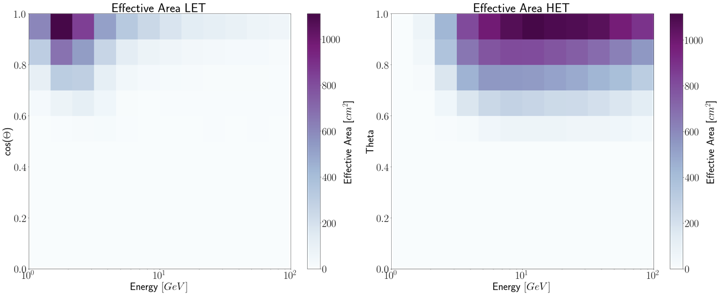
\includegraphics[scale=0.65]{effective_Area.png}
  \caption{Effective area based on the applied selection, as a function of both the incoming angle($\theta$) and energy. From left to right, the effective area for Low Energy Trigger (LET) events and the High Energy Trigger events (HET). }
  \label{eff_area}
\end{figure}


%\begin{figure}
%  \begin{center}
%    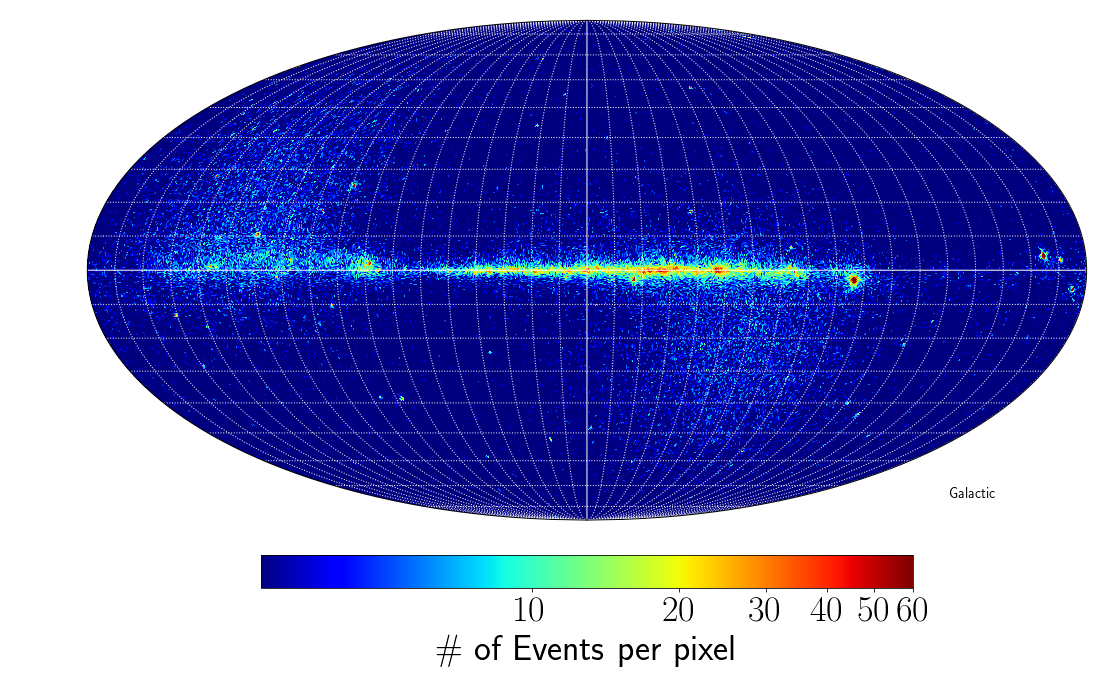
\includegraphics[scale=0.25]{map.png}
%    \caption{Skymap for 39 months of the DAMPE on-orbit measurements in survey mode. The map is plotted in a Mollweide projection in Galactic coordinates and with m. The plotted photon candidates, have raw energies from 1 GeV to 100 GeV. The map shows events  }
%    \label{map}
%  \end{center}

%\end{figure}


\section{Pulsars}

Pulsars are highly magnetized and rapidly rotating neutron stars. Neutron stars are  extremely dense objects, that  are used as  astrophysical laboratories that help to test the constant struggling relation between astrophysics, nuclear physics  and particle physics. %Pulsars are thought to be the result of Type II supernovae explosions, in order words the collapse of  of a start with a mass  $> 8 M_ {\odot} $.

In this section the methods applied  to data for the light-curve calculation and the energy spectrum are presented.



\subsection{Pulsars Folding}
The different ways to detect a pulsar are dependent on the acceptance of the instrument and on its orbit. In the case of DAMPE we do a search based on known pulsars and  then use timing models calculated by other experiments, normally in different wavelength such as radio,x-ray or even gamma  rays. The pulsar timing solutions (ephemerides) of interest in this work were all provided by David A. Smith (Private Communication, 2017).

%The algorithm to arrive to this is described in the diagram sown in Figure \ref{steps_pulsars}, in the previous the photon selection is explained. The  next step is to select the events of interests  depending on their position, for this we use the known position of sources and first apply a $3 \times 3  \text{ deg} ^2$ window around it.

From the data selected as explained in the previous section, we select events of interest for each pulsars, around their known position. The required information includes the timestamp and position of the satellite where each event is detected, and the known position in the sky for the different sources, this position is given by other experiments mainly radio searches.
This subset is then barycentered, meaning we convert the DAMPE timestamps that are given in Mission Elapsed Time (MET) to Coordinated Universal Time (UTC) to finally convert to Barycentric Dynamical Time (TDB) this is done to correct for relativistic effects related  to  time dilatation this time variations are very small but important and consider effects such as Jupiter's and the sun's orbit. To do this it is important  to have precise arrival time stamps of the photons detected and its geographical coordinates. The position of the known source also need to be precise, therefore proper motion i.e. motion of the pulsar is also considered.
Finally we  fold the TDB times with the ephemerides given by other experiments, this last step is done using the TEMPO2 software package \cite{tempo2}.   The reason to use this  type of software is that the pulsars are considered to be decelerating and this can be modeled giving rotation parameters that can be applied later  to different experiments, nevertheless the  rotation parameters can be very complex for different  pulsars in particular of those that undergo "glitches" irregular changes in the rotation parameters and TEMPO2 validity has been widely proved \cite{2catalogfermi} \cite{geminga_fermi}. Because of the need of time precision we also need to take into consideration leap seconds. Leap seconds are also taken into consideration, and since the start of the MET ($01/01/2013$) 2 leap seconds have been added.


%Consider for timing  that GPS time  doesn't  contain leap seconds. Up to know  there are 37 leap seconds  that need to be added.
%The leap seconds occur at a giving time, since the launch of DAMPE one  leap second  has been added,therefore  the corrections and time trnasformation are dpeendent  in the

\subsubsection{Light-curve Validation}
Validation of the pulsars detection is required, for this we perform a statistical test that will  allows to understand the significance of  the pulsation, the statistical test used is called the H-test and it is widely used in the pulsar community.
%The  second consist in a direct comparison with the Fermi experiment. Fermi is a dedicated $\gamma$-ray experiment  and has been in orbit for over  10 years,  during this time two pulsar catalogues have been published with over 100 pulsars, all of this with searches from 100 MeV to energies above 100 GeV.

This test has the capability to evaluate both the timing model and the quality of the data used.  The H-test was presented for its application in the use of pulsars in 1989,a further  modification of this test was presented in \cite{h-test}.
The test consists in searching for uniformity in the circle.  Meaning the search for  periodicity on  a phase. From the H-Test we obtain an H-Value that can be translated to a probability.





%For being able to compute the phase we use the pulsar timing solutions (ephemeris) of interest in combination with the timestamp and position recorded for each event, and the known position in the sky for the different sources, normally measured by other experiments. In this case all the ephemerides  were provided by David A. Smith (Private Communication, 2017).

\subsection{Energy Spectrum}
From the  events detected we require to convert between the measured distribution of energy and direction measured by DAMPE to the truth flux of gamma-rays on the sky. In order to do this we use the Instruments Response Functions (IRFs). The IRFs  can be  separated into three parts: the effective area $A_{eff}$, the Point Spread Function PSF and the Energy Redistribution Function ERF. To produce the response we depend on reliable GEANT4 simulations of the instrument.

The IRF is defined as below:

\begin{equation}
IRF=A_{eff}(E,\theta)\times{PSF}(\delta\theta;E,\theta)\times ERF (E';E,\theta)
\end{equation}

The Effective area is therefore given as function of the truth energy and truth theta. To calculate the effective area we use the following formula
\begin{equation}
\frac{\textbf{Events Passed the Selection}}{\textbf{All Events Generated}}\times {\textbf{Generation Area}}
\end{equation}
The generation area will depend on the  MC and depending on the MC we use, the integration on the solid angle will also vary. The effective Area results can be observed on Figure \ref{eff_area}.

For the energy redistribution function we define the measured energy as function of the true energy and true incoming angle ($\theta$). Once this is done, the correction is applied by using a Bayesian iterative method, where the response matrix is obtained from the normalize redistribution function.

Finally, we also need to calculate live time. For this we applied a $ \pm 60^{\circ}$ window around the source of interest and collect the amount of seconds the DAMPE has spend in this area. The choice of the window is given the Field of View of DAMPE at anytime.


\section{Results}
In this  sections  the  results of the analyzed pulsars will be presented. At the moment more than 20 pulsars have been  studied with DAMPE data set, nevertheless here only five are presented. The pulsars presented for this work were selected based on the number of events detected for each pulsar. The chosen pulsars have the most counts  in a  two year observation period within a ROI of $1^\circ$ around the known position of the source. However the analysis is applied  for a ROI of $3^\circ$,and for the folding of the pulsars we use 2 years of data, from the 1st of January 2016 till the 1st of January 2018.  Nevertheless for the  energy spectrum we use 39 months of data, from the 1st of January 2016 til the  31st of March 2019. The current limitation on the 2 years of data for the  light-curve calculation is due to the validity of the ephemerides.

%% this area is too big to be able to determine if the detected photons are coming from one source or  multiple sources this is the case mainly when the source is located in the galactic plane,therefore a smaller area is consider to reduce the contamination by other sources.
 The reason for this is that  the background or other $\gamma$-ray sources will not contribute  to the phase shape but with a bigger window it increases our statistics that help us create more reliable  light curves. The five pulsars presented here, have a sigma greater than five, confirming the detection of the pulsation.

The five pulsars studied were Vela, Geminga, J1709-4429, Crab and J0007+73703, and the results of the analysis can be observed in Figures \ref{vela}, \ref{geminga}, \ref{j1709}, \ref{crab} and \ref{j0007} respectively.

%%%J0835-4510
\begin{figure}
\centering
\subfloat[Light-curve]{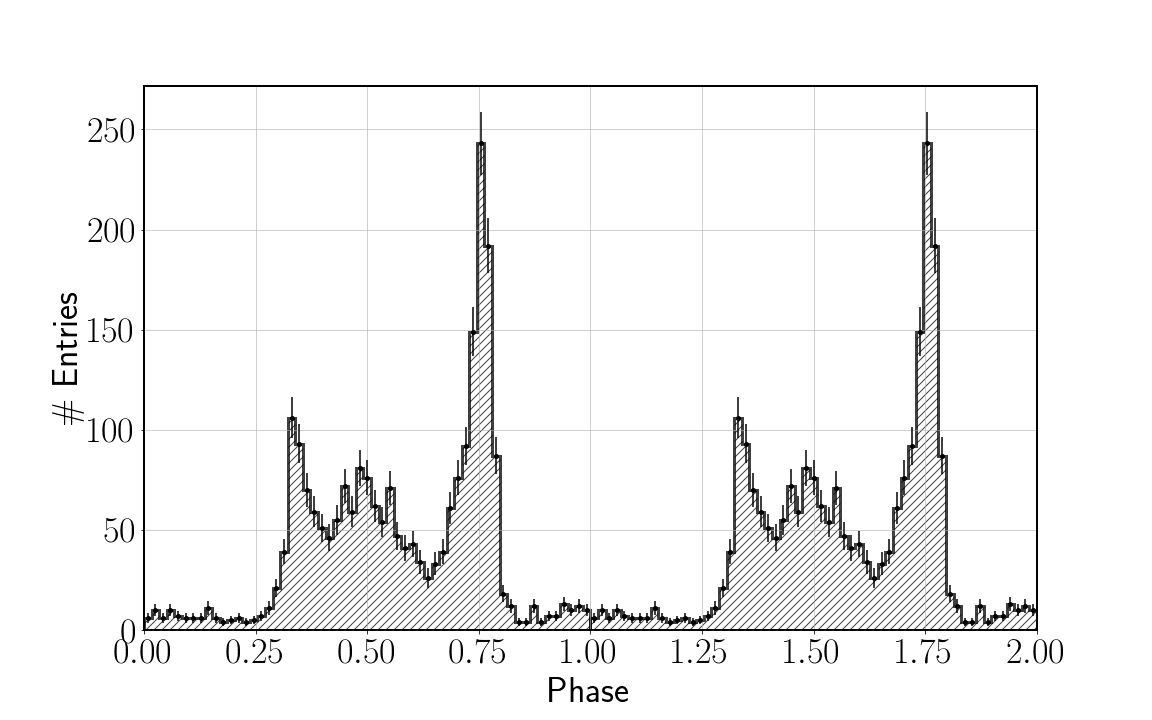
\includegraphics [width=0.5\textwidth,, keepaspectratio]{J0835-4510phase_3deg.png}}
\subfloat[Energy Flux]{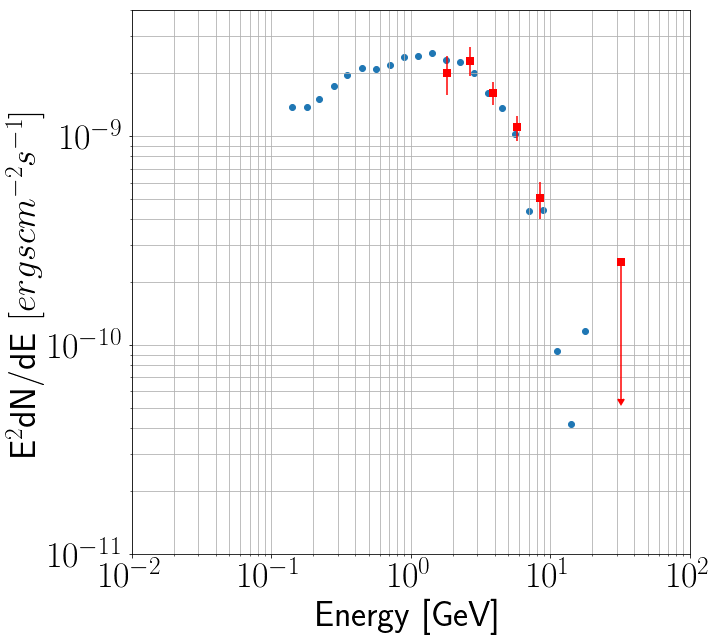
\includegraphics [width=0.3\textwidth,, keepaspectratio]{flux_vela.png}}
%%\hspace{\fill}
%%\centering
%\subfloat[]{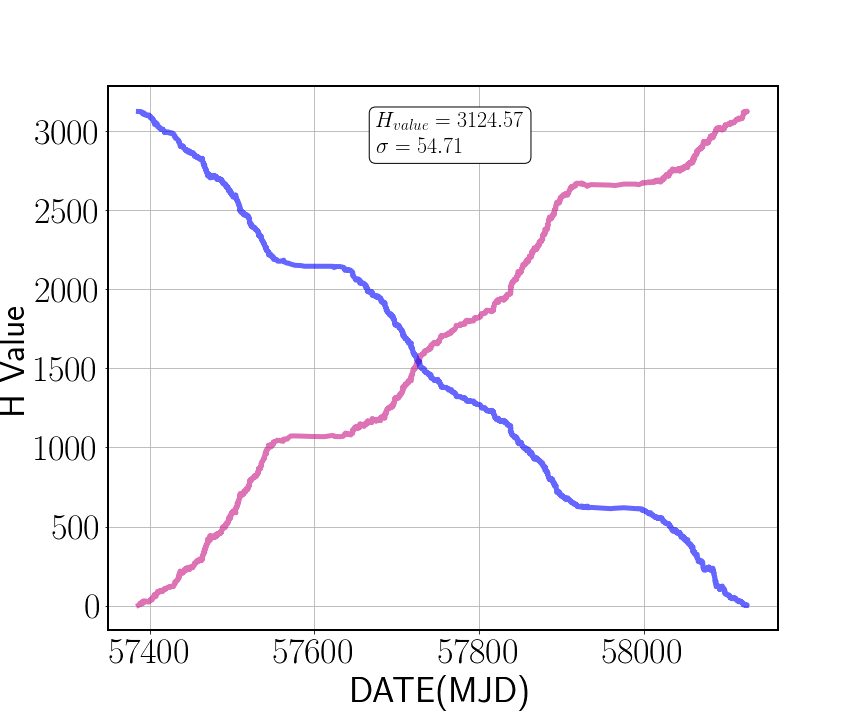
\includegraphics [width=0.3\textwidth, keepaspectratio]{J0835-4510H_value_3deg.png}}
\subfloat[]{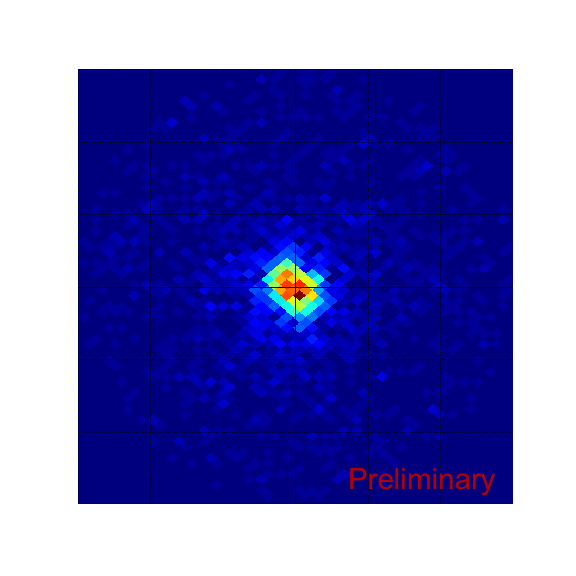
\includegraphics [width=0.3\textwidth, keepaspectratio]{J0835-4510position.png}}
%\includegraphics[scale=0.7]{images/j0007.png}
\caption{Results of the pulsar J0835-4510, a)  shows its characteristic  light curve. The pulsating detection has a $ \sigma =54.71$ b)Energy Spectrum as measured for this analysis by DAMPE in red from 2 GeV to 100 GeV. The blue points correspond to FERMI measurements taken from \cite{vela_fermi}. }\label{vela}
\end{figure}

%%J0633+1746
\begin{figure}
\centering
\subfloat[Phase information]{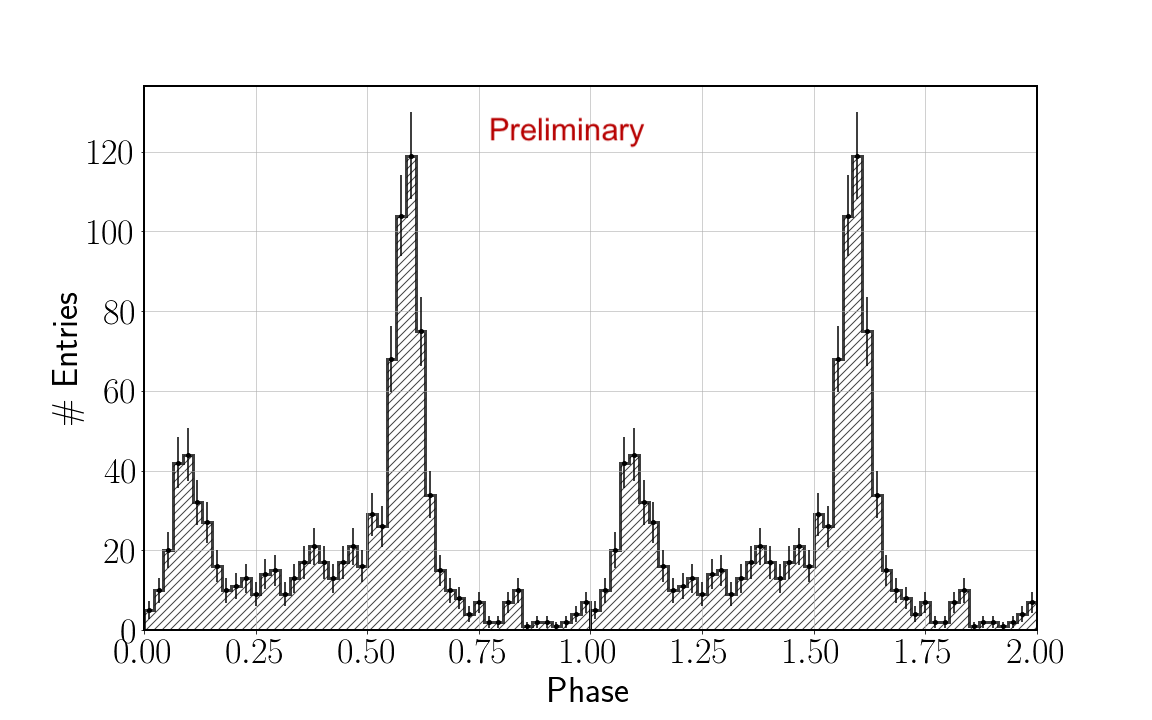
\includegraphics [width=0.5\textwidth,, keepaspectratio]{J0633+1746phase_3deg.png}}
\subfloat[Energy Flux]{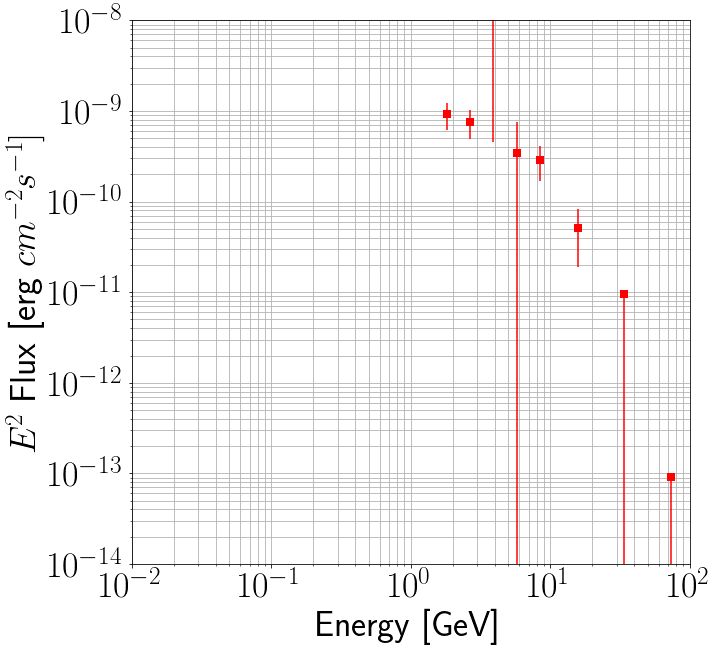
\includegraphics [width=0.3\textwidth,, keepaspectratio]{flux_geminga.png}}
%\hspace{\fill}
%\centering
%\subfloat[]{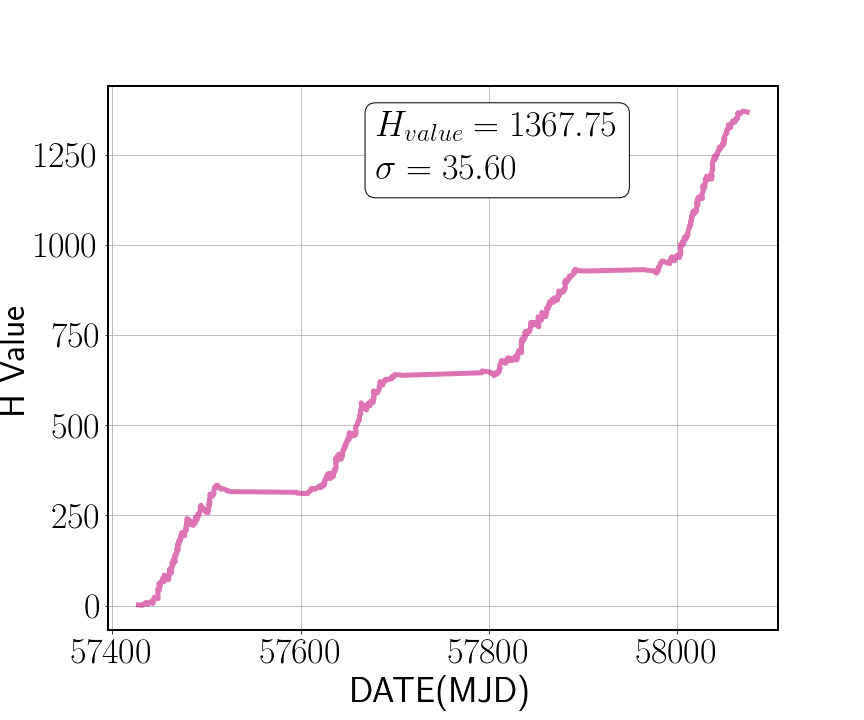
\includegraphics [width=0.3\textwidth, keepaspectratio]{J0633+1746H_value_3deg.png}}
\subfloat[]{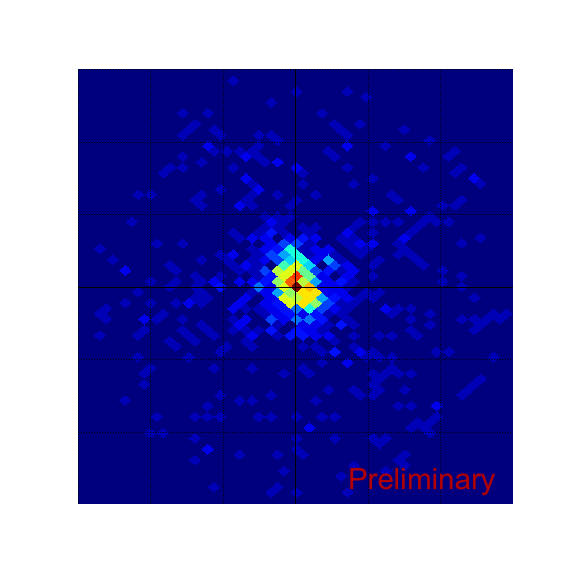
\includegraphics [width=0.3\textwidth, keepaspectratio]{J0633+1746position.png}}
%\includegraphics[scale=0.7]{images/j0007.png}

\caption{Results of the pulsar J0633+1746 also known as Geminga, a)  shows its characteristic  light curve. b) Energy Spectrum from 2GeV to 100 GeV.}\label{geminga}
\end{figure}


%%J1709-4429
\begin{figure}
%\centering
\subfloat[Phase information]{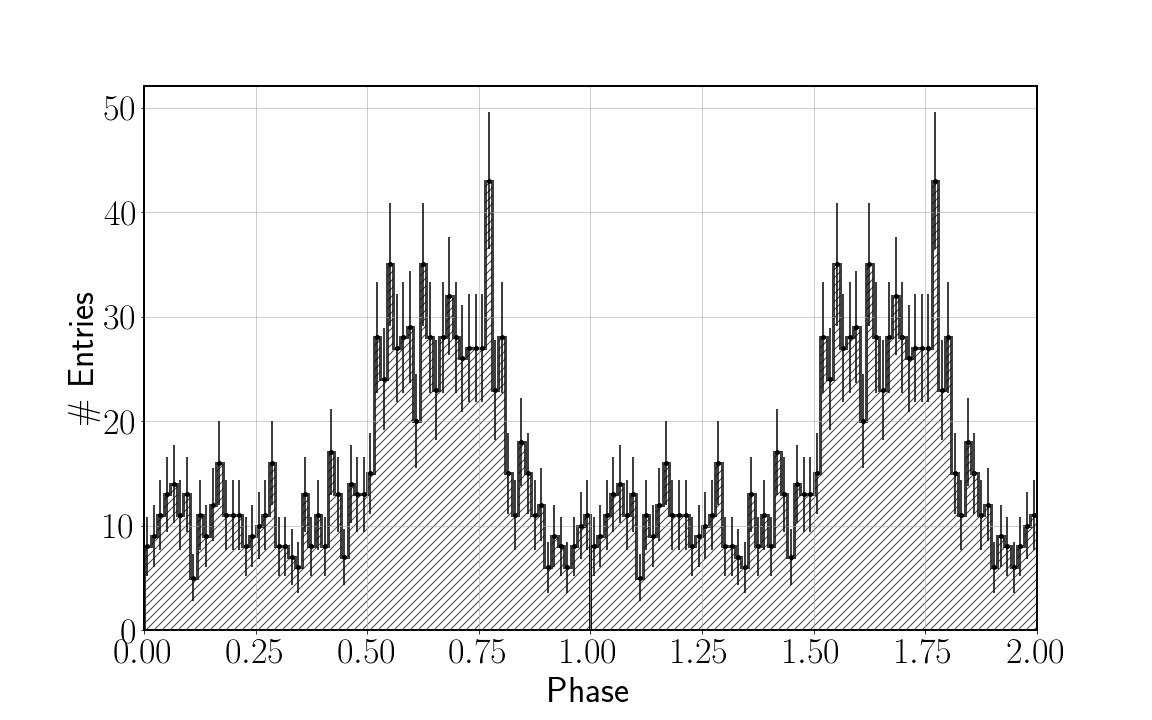
\includegraphics [width=0.5\textwidth,, keepaspectratio]{J1709-4429phase_3deg.png}}
\subfloat[Energy Flux]{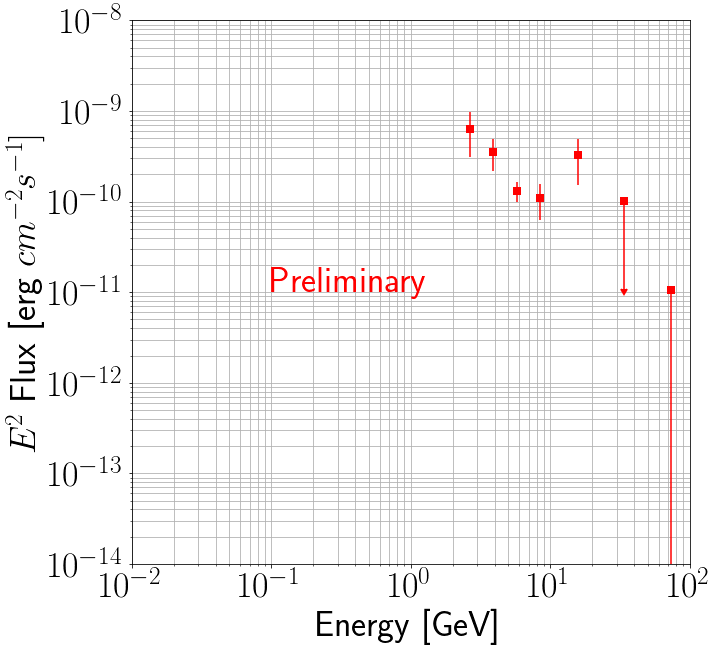
\includegraphics [width=0.3\textwidth,, keepaspectratio]{flux_J1709-4429.png}}
%\hspace{\fill}
%\centering
%\subfloat[]{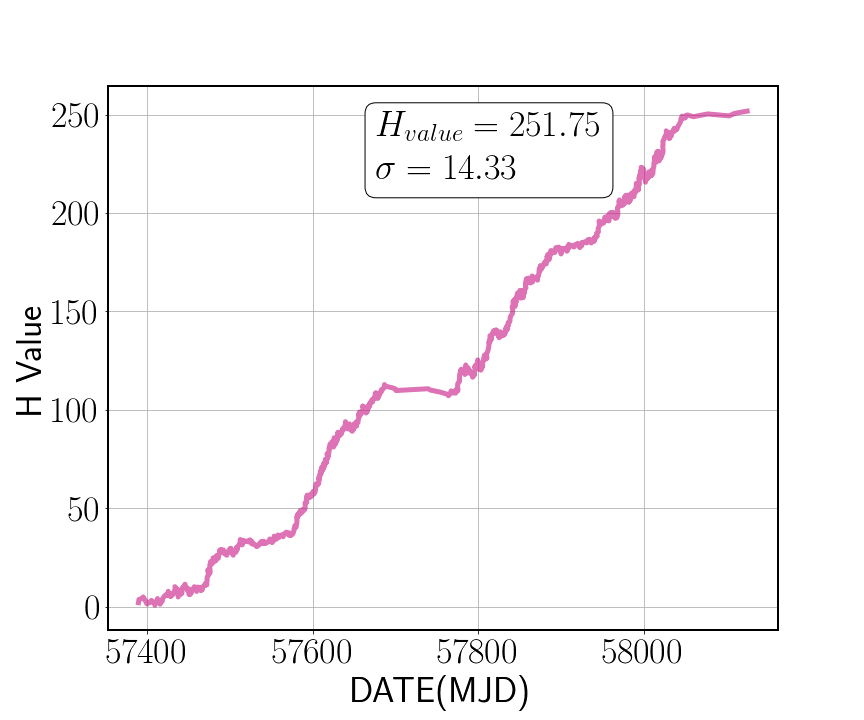
\includegraphics [width=0.3\textwidth, keepaspectratio]{J1709-4429H_value_3deg.png}}
\subfloat[Image]{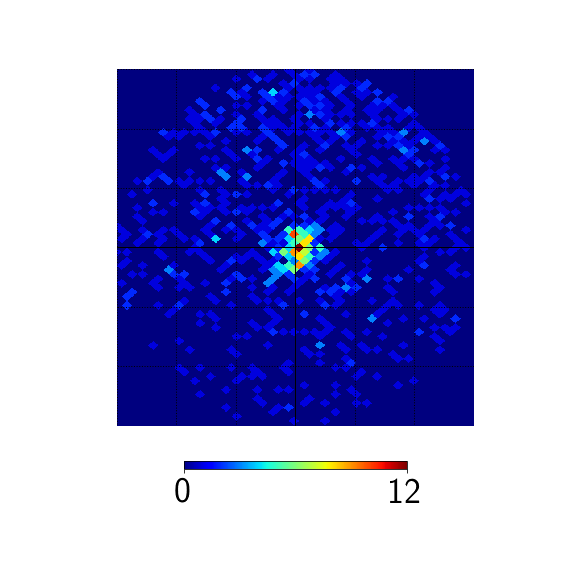
\includegraphics [width=0.3\textwidth, keepaspectratio]{J1709-4429position.png}}
%\includegraphics[scale=0.7]{images/j0007.png}
\caption{Results of the pulsar J1709-4429, a)  shows its characteristic  light curve. b) Energy Spectrum from 2GeV to 100 GeV.}\label{j1709}
\end{figure}


%%J0534+2200
\begin{figure}
\centering
\subfloat[Phase information]{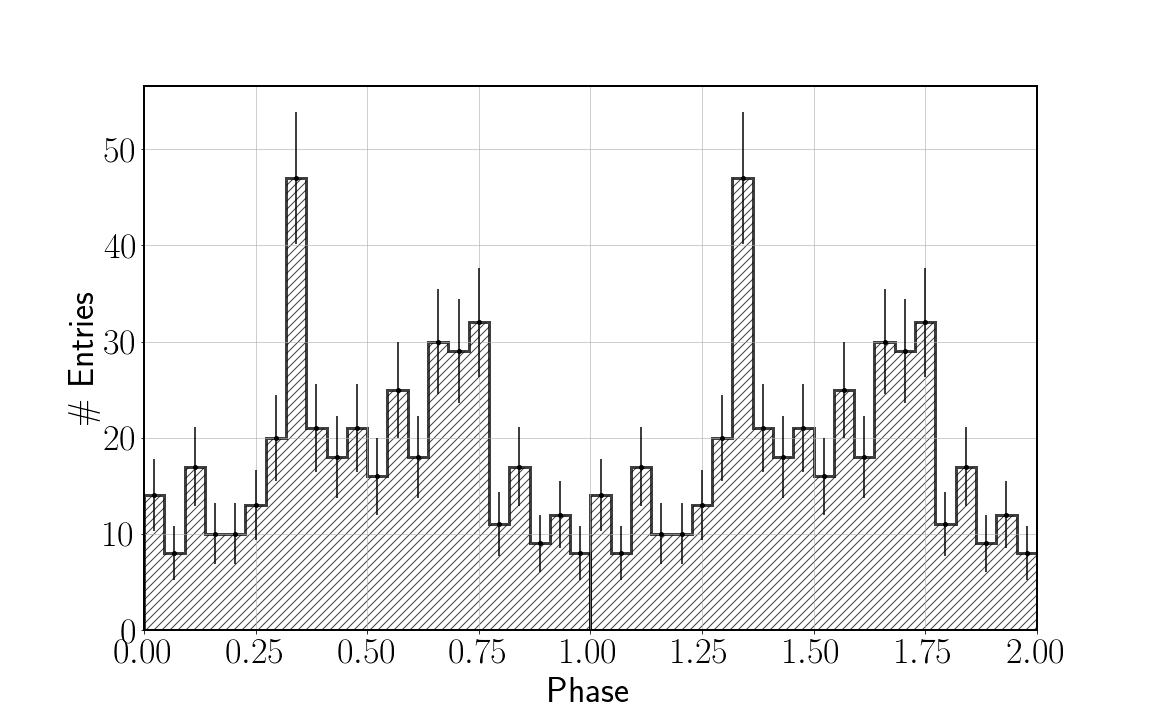
\includegraphics [width=0.5\textwidth,, keepaspectratio]{J0534+2200phase_3deg.png}}
\subfloat[Energy Flux]{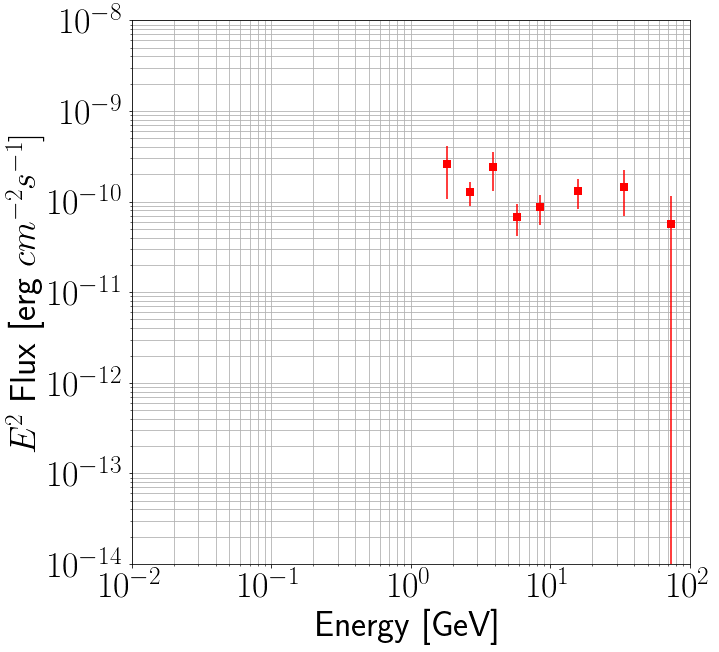
\includegraphics [width=0.3\textwidth,, keepaspectratio]{flux_crab.png}}
%\hspace{\fill}
%\centering
%\subfloat[]{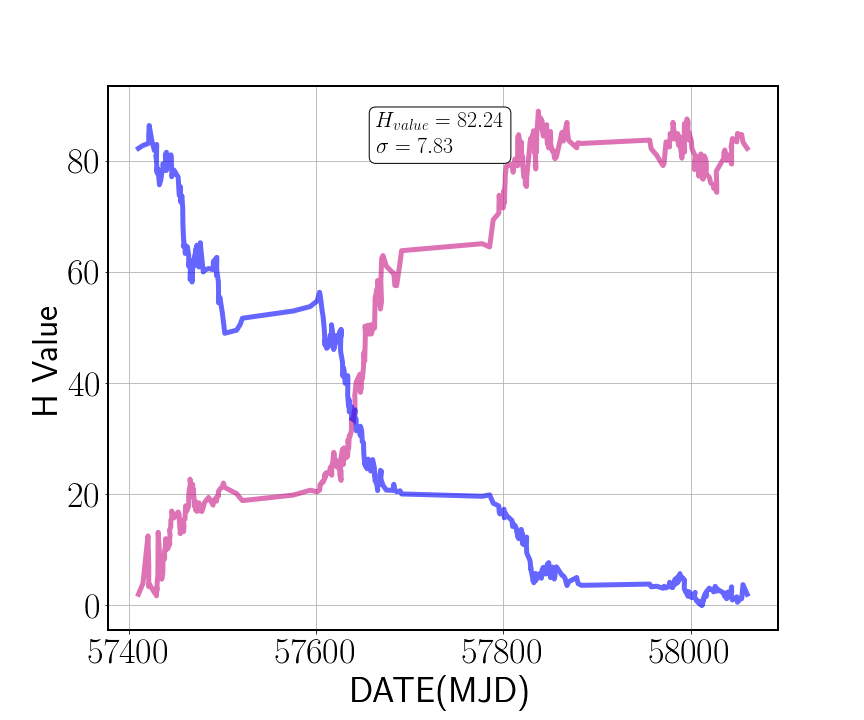
\includegraphics [width=0.3\textwidth, keepaspectratio]{J0534+2200H_value_3deg.png}}
\subfloat[]{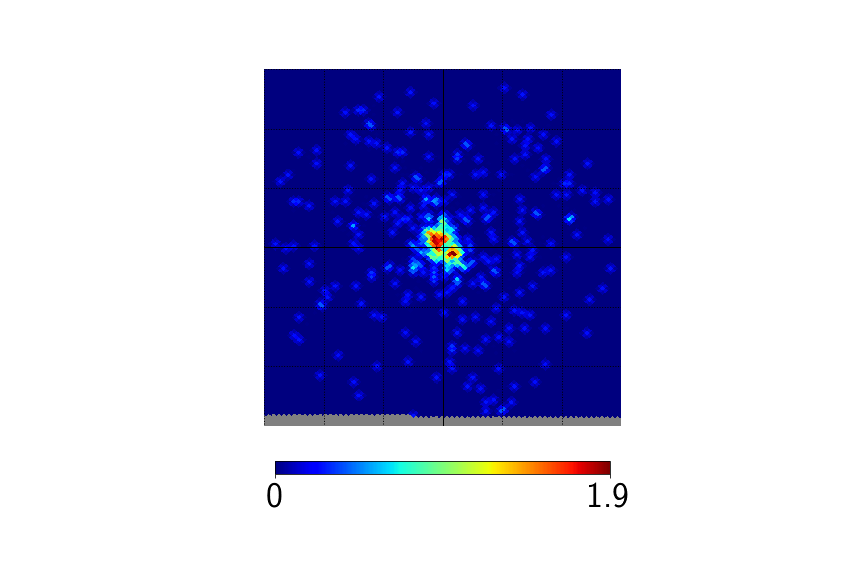
\includegraphics [width=0.3\textwidth, keepaspectratio]{J0534+2200position.png}}
%\includegraphics[scale=0.7]{images/j0007.png}
\caption{Results of the Crab (J0534+2200), a)  shows its characteristic  light curve. b) Energy Spectrum from 2 GeV to 100 GeV. For the energy spectrum we need to consider that this will also contain the nebula and not just the pulsar spectrum}\label{crab}
\end{figure}

%%J0007+7303
\begin{figure}
\centering
\subfloat[Phase information]{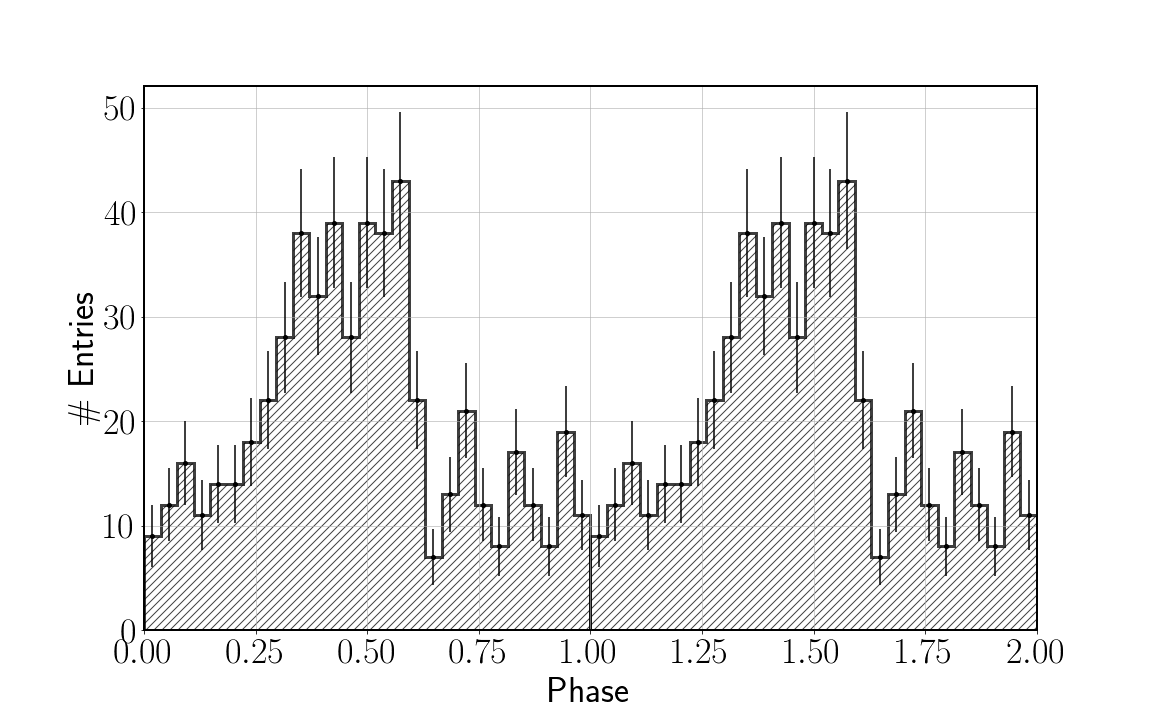
\includegraphics [width=0.5\textwidth,, keepaspectratio]{J0007+7303phase_3deg.png}}
\subfloat[Energy Flux]{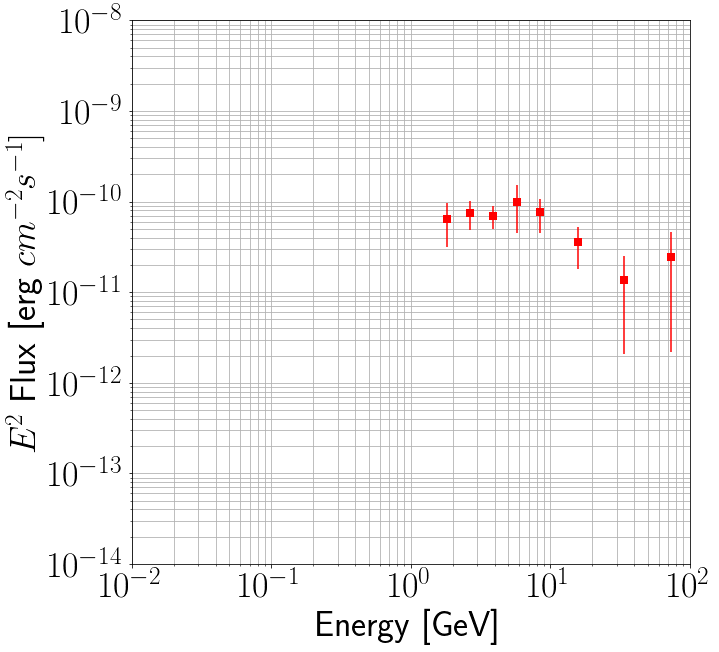
\includegraphics [width=0.3\textwidth,, keepaspectratio]{flux_j0007+7303.png}}
%\hspace{\fill}
%\centering
%\subfloat[]{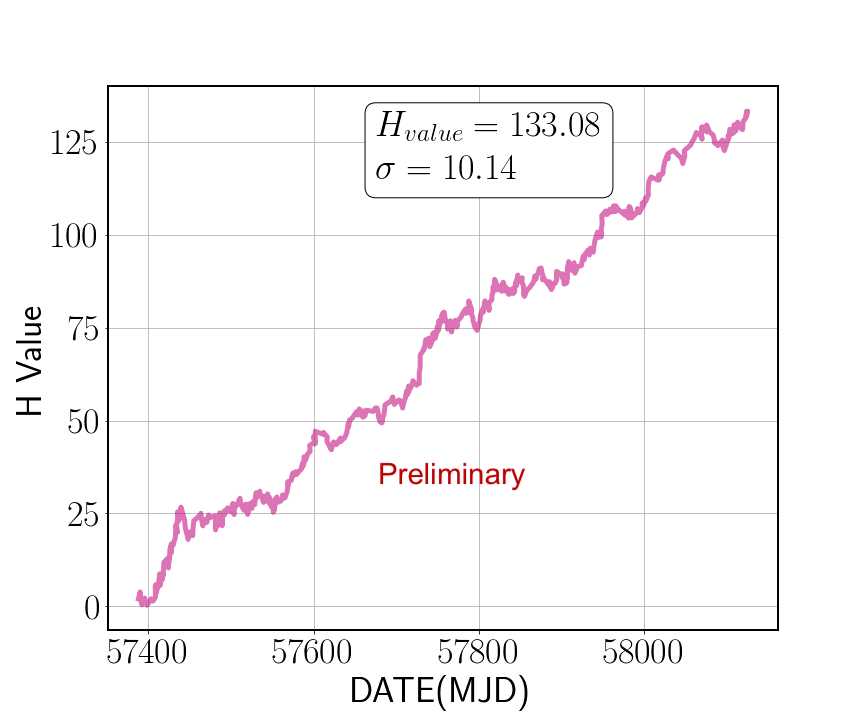
\includegraphics [width=0.3\textwidth, keepaspectratio]{J0007+7303H_value_3deg.png}}
\subfloat[]{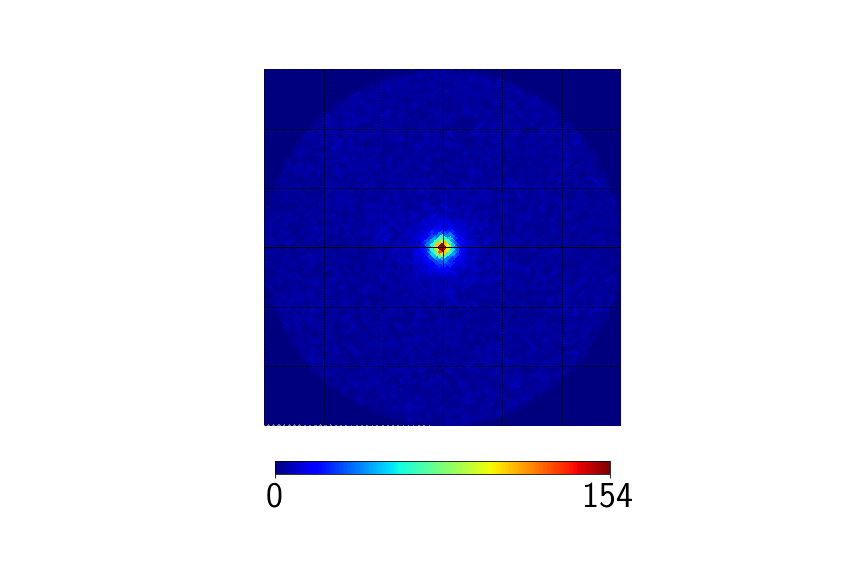
\includegraphics [width=0.3\textwidth, keepaspectratio]{J0007+7303position.png}}
%\includegraphics[scale=0.7]{images/j0007.png}
\caption{Results of the pulsar J0007+7303, a)  shows its characteristic  light curve. b) Energy Spectrum from 2GeV to 100 GeV.}
\label{j0007}
\end{figure}




\section{Conclusions and future scope}
With 24 months of  data, we showed DAMPE's ability to measure gamma-rays in an energy range from 1-100GeV.
We also show its timing capabilities for the identification and analysis of pulsars.
In the future we aim to perform spectral analysis in the pulse and off-pulse regions, observe the evolution of light curves  as a function of energy.
We also have shown the broad possibilities for research and study of gamma-ray sources such as the galactic plane, SNRs, AGNs, GRBs among others.




\section{Acknowledgements}
MMS expresses her gratitude to David A. Smith for providing the ephemerides applied for this analysis along with invaluable discussions that have help further this work.



\begin{thebibliography}{99}

\bibitem{vela_fermi}
  A.~A.~Abdo {\it et al.} [Fermi-LAT Collaboration],
  ``Fermi LAT Observations of the Vela Pulsar,''
  Astrophys.\ J.\  {\bf 696}, 1084 (2009)
  %%doi:10.1088/0004-637X/696/2/1084
  [arXiv:0812.2960 [astro-ph]].
\bibitem{geminga_fermi}
  A.~A.~Abdo {\it et al.} [Fermi-LAT Collaboration],
  ``Fermi LAT observations of the Geminga pulsar,''
  Astrophys.\ J.\  {\bf 720}, 272 (2010)
  %%doi:10.1088/0004-637X/720/1/272
  [arXiv:1007.1142 [astro-ph.HE]].
\bibitem{j0007}
  A.~A.~Abdo {\it et al.},
  ``PSR J0007+7303 in the CTA1 SNR: New Gamma-ray Results from Two Years of Fermi-LAT Observations,''
  Astrophys.\ J.\  {\bf 744}, 146 (2012)
  %%doi:10.1088/0004-637X/744/2/146
  [arXiv:1107.4151 [astro-ph.HE]].
\bibitem{2catalogfermi}
  A.~A.~Abdo {\it et al.} [Fermi-LAT Collaboration],
  ``The Second Fermi Large Area Telescope Catalog of Gamma-ray Pulsars,''
  Astrophys.\ J.\ Suppl.\  {\bf 208}, 17 (2013)
  %%doi:10.1088/0067-0049/208/2/17
  [arXiv:1305.4385 [astro-ph.HE]]

 \bibitem{h-test}
de Jager, O.C, Büsching, I
''The H-test probability distribution revisited: Improved sensitivity''
    arxiv.:005.4867
\bibitem{tempo2}
{{Hobbs}, G.~B. and {Edwards}, R.~T. and {Manchester}, R.~N.},
"{TEMPO2, a new pulsar-timing package - I. An overview}",
{astro-ph/0603381},

\bibitem{dampe_mission}
  J.~Chang {\it et al.} [DAMPE Collaboration],
  ``The DArk Matter Particle Explorer mission,''
  arXiv:1706.08453 [astro-ph.IM].

\bibitem{chandra}
J.~P.~Halpern, E.~V.~Gotthelf, F.~Camilo, D.~J.~Helfand and S.~M.~Ransom,
 ``X-ray, radio, and optical observations of the putative pulsar in the supernova remnant CTA 1,''
  Astrophys.\ J.\  {\bf 612}, 398 (2004)
  %%doi:10.1086/422409
  [astro-ph/0404312].

\bibitem{zunlei}
Xu, Z.{\it et al.},
"An algorithm to resolve γ-rays from charged cosmic rays with DAMPE"
arxiv.:1712.02939


\end{thebibliography}



\end{document}
